The \texttt{WorldSpaceCanvas} is a canvas object, which in Unity serves as a container for other user interface elements, such as buttons and input fields, 
and is rendered in world space. It is thus diegetic and exists there like other 3D objects.

In applications that don't utilize virtual reality, canvases and other UI elements are usually non-diegetic (i.e they don't exist within the game world), 
and in 2D and drawn directly to the screen space (as opposed to world space) using x- and y-coordinates.
With this approach one can specify e.g.~a position by its x- and y-coordinate, where \{0, 0\} usually represents the top-left of the display.
This changes in virtual reality applications, as the user's eyes are unable to focus on the screen space. An analogy to this would be to 
ask the user to read a letter while holding it 2-3 centimeters from their eyes. Because of this, elements appearing on the screen space is not rendered
in unity while running it with the virtual reality SDKs. 

\begin{figure}%[h!] %[H]
	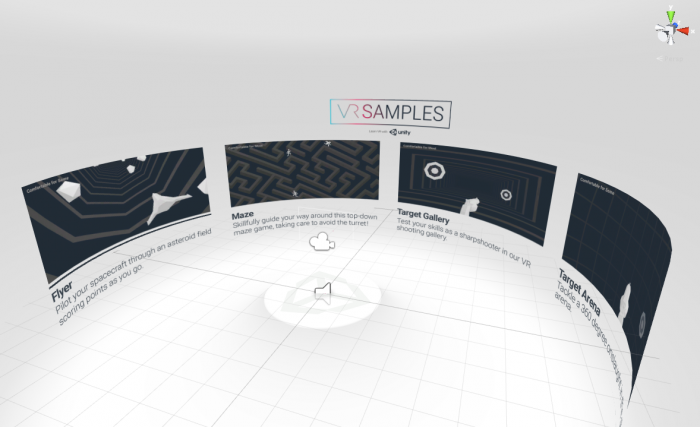
\includegraphics[width=\linewidth]{pictures/unity_vr_menu.png}
	\caption[An example of world-space (diegetic) user interfaces]{An example of world-space (diegetic) user interfaces~\citep{Unity}.}
	\label{fig:unity_vr_menu}
\end{figure} 

Another reason why the canvas is rendered in world space, and also the reason why this is the case in desktop mode, is because of our touch interaction.
To enable the user to click on buttons using his or her hands, the user interface must also exist in world-space so a collision can occur between the desired 
button and the hand models (that mimic the users hand). 

\texttt{WorldSpaceCanvas} is thus rendered in the world space, and is always positioned 0.8 unity meters (i.e the virtual representation of a meter in unity) 
in front of the user. The game object is thus always in the center of the camera, but is only visible and enabled when the user is editing an annotation. 
One issue with this approach is "clipping", i.e that the annotation form visually collides with another object (e.g.~the tank model or an annotation sphere) thus
obstructing it from view. To combat this \texttt{WorldSpaceCanvas} has a box-shaped collider component, which covers the canvas as well as the area between the canvas and the camera, 
and a script called \texttt{CanvasCollider}, which keeps track of objects that's within the collider component. When the user wish to edit an annotation, and the 
\texttt{AnnotationForm} and \texttt{Hoverkey} becomes active, the objects within the canvas' collider is disabled, thus hiding objects that could potentially
obstruct the whole, or parts of, the canvas. The objects are enabled again once the users is done editing the annotation (i.e when the user clicks "submit", "cancel" or "delete").

\begin{figure}%[h!] %[H]
	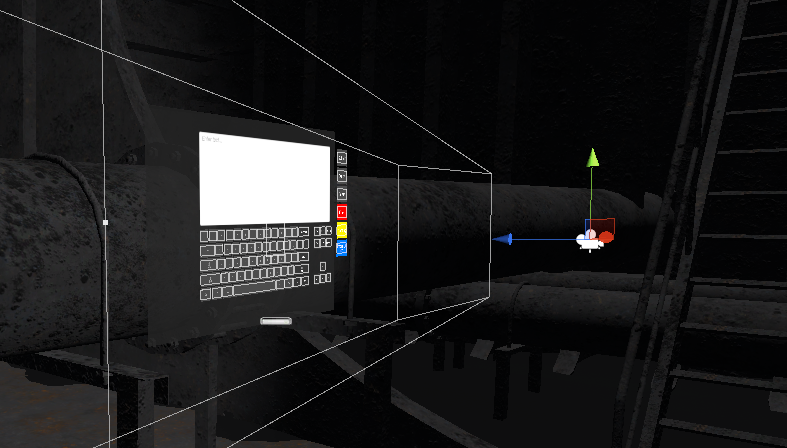
\includegraphics[width=\linewidth]{pictures/screenshots/canvas/worldspacecanvas_scene.png}
	\caption[The \texttt{WorldSpaceCanvas} as seen in the Unity Scene View]{The \texttt{WorldSpaceCanvas} as seen in the Unity Scene View.}
	\label{fig:worldspacecanvas_scene}
\end{figure} 

\begin{figure}%[h!] %[H]
	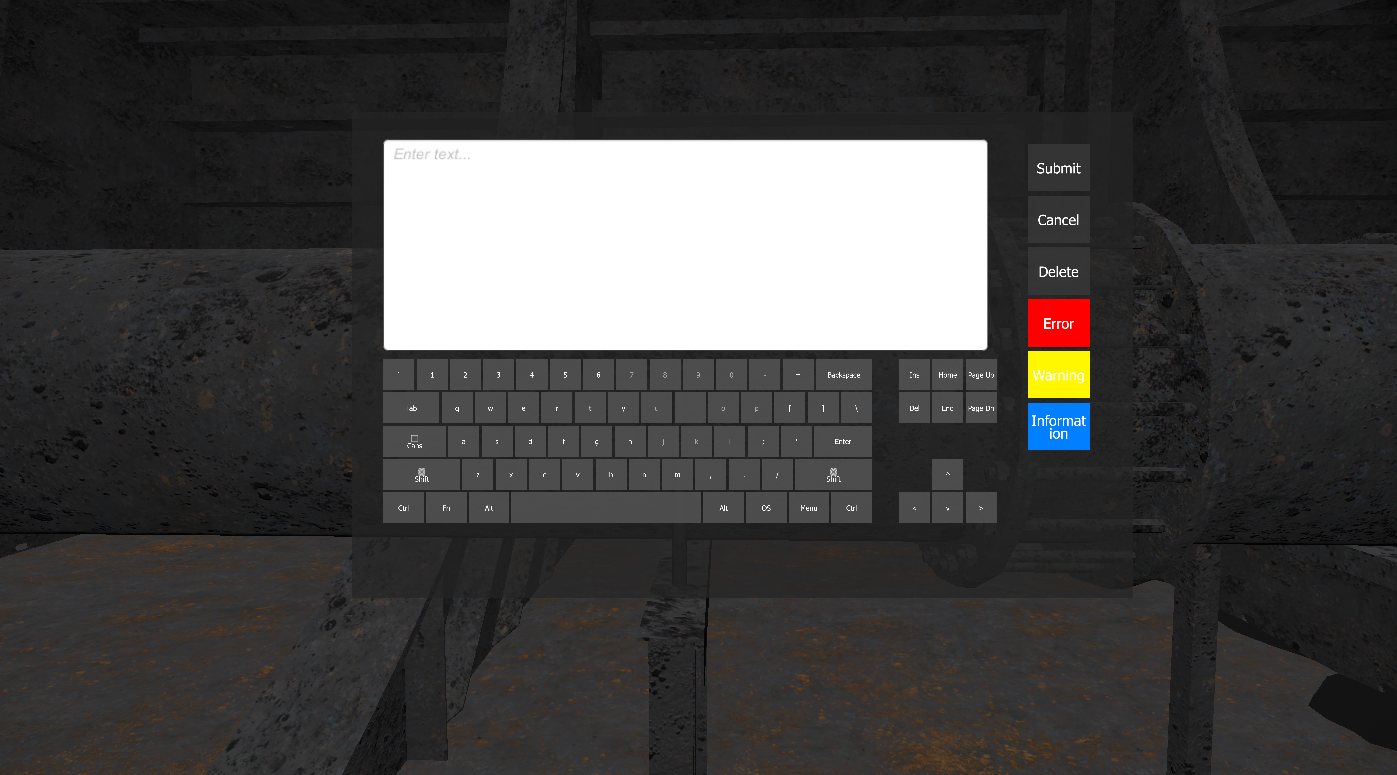
\includegraphics[width=\linewidth]{pictures/screenshots/canvas/worldspacecanvas_ingame.png}
	\caption[The \texttt{WorldSpaceCanvas} as seen in the Unity Game View]{The \texttt{WorldSpaceCanvas} as seen in the Unity Game View.}
	\label{fig:worldspacecanvas_ingame}
\end{figure} 

The \texttt{WorldSpaceCanvas} has two child game objects: \texttt{AnnotationForm} and \texttt{Hoverkey}. 
\texttt{AnnotationForm} currently only contains a inputfield-object and a background rectangle, but can in future iteration grow to 
contain other user interaction elements. The \texttt{Hoverkey} game object represents the touch keyboard and is part of the HoverUI-kit.
In addition to the keyboard six other similar buttons are also present: Submit, Cancel, Delete, Error, Warning and Information (see~\vref{fig:worldspacecanvas_ingame}).